\chapter{Технологический раздел}

\section{Выбор языка и среды программирования}
Для написания программного кода использовался язык программирования C \cite{bib:4}, так как в реализации использовались структуры ядра Linux, а исходный код ядра написан на C.

В качестве среды программирования использовалась среда CLion, так как она предоставляет широкий выбор плагинов для работы с кодом на языке C.

\section{Реализация алгоритмов мониторинга информации о процессах}

В листинге \ref{algo1} представлен код алгоритма вывода информации о процессах в файл /proc.
\begin{lstlisting}[label=algo1,caption=Реализация алгоритма вывода информации о процессах]
static char log[LOG_SIZE] = { 0 };
int was_read = 1;
static ssize_t my_read(struct file *filep, char __user *buf, size_t count, loff_t *offp)
{
    was_read = !was_read;
    if (was_read)
        return 0;
        
    memset(log, 0, LOG_SIZE);
    print_tasks();
    ssize_t logLen = strlen(log);
    printk(KERN_INFO "read called\n");

    if (copy_to_user(buf, log, logLen))
    {
        printk(KERN_ERR "copy_to_user error\n");
        return -EFAULT;
    }

    return logLen;
}
\end{lstlisting}
В листинге \ref{algo2} представлен код алгоритма получения информации о процессах из структур ядра.
\begin{lstlisting}[label=algo2,caption=Реализация алгоритма получения информации о процессах из структур ядра]
#define TEMP_STRING_SIZE 512
#define LOG_SIZE 256 * 1024
static char log[LOG_SIZE] = { 0 };
static struct proc_dir_entry *proc_file;
void print_tasks(void)
{
    struct task_struct *task;
    char temp[TEMP_STRING_SIZE];
    task = &init_task;
    memset(temp, 0, TEMP_STRING_SIZE);
    snprintf(temp, TEMP_STRING_SIZE,
             "%-5s %15s %6s %4s %5s %5s %5s %3s %6s %15s %15s %16s %16s %16s %6s %15s %18s %11s\n",
             "PID","name", "state", "prio", "sprio",
             "nprio", "rprio", "cpu", "policy",
             "utime", "stime", "exec_start","sum_exec_runtime",
             "vruntime", "pcount", "run_delay", "last_arrival", "last_queued");
    strcat(log, temp);
    for_each_process(task)
    {
        memset(temp, 0, TEMP_STRING_SIZE);
        snprintf(temp, TEMP_STRING_SIZE,
                 "%-5d %15s %6d %4d %5d %5d %5d %3d %6d %15lld %15lld %16lld %16lld %16lld %6lu %15llu %18llu %11llu\n",
                 task->pid, task->comm, task->__state,
                 task->prio, task->static_prio, task->normal_prio, task->rt_priority,
                 task->cpu, task->policy,
                 task->utime, task->stime,
                 task->se.exec_start, task->se.sum_exec_runtime, task->se.vruntime,
                 task->sched_info.pcount, task->sched_info.run_delay, task->sched_info.last_arrival, task->sched_info.last_queued);

        if (strlen(temp) + strlen(log) < LOG_SIZE)
            strcat(log, temp);
        else
            printk(KERN_ERR "max log size was exceeded!\n");
    }
}
\end{lstlisting}

В листинге \ref{algo3} представлен код алгоритма получения информации о процессах из файла в /proc в пространстве пользователя.
\begin{lstlisting}[label=algo3,caption=Реализация алгоритма получения информации о процессах из файла в /proc в пространстве пользователя]
...
#include <...>
#define SIZE_OF_LOG 8192
#define ERROR_COMMAND_EXEC 1
#define TIMES 100
#define DELAY 1
int main(int argc, char *argv[])
{
    FILE *filePointer = NULL;
    char log[SIZE_OF_LOG] = {'\0'};
    for (int i = 0; i < TIMES; i++)
    {
        filePointer = popen("cat /proc/analyzer", "r");
        if (filePointer == NULL)
        {
            printf("Error: can't execute cat for process analyzer");
            return ERROR_COMMAND_EXEC;
        }
        while (fgets(log, sizeof(log), filePointer) != NULL)
        {
            printf("%s", log);
            fgets(log, sizeof(log), filePointer);
            printf("%s", log);
        }
        pclose(filePointer);
        sleep(DELAY);
    }
    return EXIT_SUCCESS;
}
...
\end{lstlisting}

В листинге \ref{lstcode1} представлен полный код модуля ядра, предоставляющего файл в /proc для мониторинга информации о процессах .
\begin{lstlisting}[label=lstcode1,caption=Код модуля ядра]
#include <...>
MODULE_LICENSE("GPL");
MODULE_AUTHOR("Varlamova Ekaterina");
#define PROC_FS_NAME "analyzer"
#define TEMP_STRING_SIZE 512
#define LOG_SIZE 256 * 1024
static char log[LOG_SIZE] = { 0 };
static struct proc_dir_entry *proc_file;
int was_read = 1;
void print_tasks(void)
{
    struct task_struct *task;
    char temp[TEMP_STRING_SIZE];
    task = &init_task;
    memset(temp, 0, TEMP_STRING_SIZE);
    snprintf(temp, TEMP_STRING_SIZE,
             "%-5s %15s %6s %4s %5s %5s %5s %3s %6s %15s %15s %16s %16s %16s %6s %15s %18s %11s\n",
             "PID","name", "state", "prio", "sprio",
             "nprio", "rprio", "cpu", "policy",
             "utime", "stime", "exec_start","sum_exec_runtime",
             "vruntime", "pcount", "run_delay", "last_arrival", "last_queued");
    strcat(log, temp);
    for_each_process(task)
    {
        memset(temp, 0, TEMP_STRING_SIZE);
        snprintf(temp, TEMP_STRING_SIZE,
                 "%-5d %15s %6d %4d %5d %5d %5d %3d %6d %15lld %15lld %16lld %16lld %16lld %6lu %15llu %18llu %11llu\n",
                 task->pid, task->comm, task->__state,
                 task->prio, task->static_prio, task->normal_prio, task->rt_priority,
                 task->cpu, task->policy,
                 task->utime, task->stime,
                 task->se.exec_start, task->se.sum_exec_runtime, task->se.vruntime,
                 task->sched_info.pcount, task->sched_info.run_delay, task->sched_info.last_arrival, task->sched_info.last_queued);
        if (strlen(temp) + strlen(log) < LOG_SIZE)
            strcat(log, temp);
        else
            printk(KERN_ERR "max log size was exceeded!\n");
    }
}
static ssize_t my_read(struct file *filep, char __user *buf, size_t count, loff_t *offp)
{
    was_read = !was_read;
    if (was_read)
        return 0;
    memset(log, 0, LOG_SIZE);
    print_tasks();
    ssize_t logLen = strlen(log);
    printk(KERN_INFO "read called\n");
    if (copy_to_user(buf, log, logLen))
    {
        printk(KERN_ERR "copy_to_user error\n");
        return -EFAULT;
    }
    return logLen;
}
static int my_open(struct inode *spInode, struct file *spFile)
{
    printk(KERN_INFO "open called\n");
    return 0;
}
static int my_release(struct inode *spInode, struct file *spFile)
{
    printk(KERN_INFO "release called\n");
    return 0;
}
static struct proc_ops ops = {
        proc_read : my_read,
        proc_open: my_open,
        proc_release: my_release
};
static int __init md_init(void)
{
    if (!(proc_file = proc_create(PROC_FS_NAME, 0666, NULL, &ops)))
    {
        printk(KERN_ERR "proc_create error\n");
        return -EFAULT;
    }

    printk(KERN_INFO "module loaded\n");

    return 0;
}
static void __exit md_exit(void)
{
    remove_proc_entry(PROC_FS_NAME, NULL);
    printk(KERN_INFO "module exited\n");
}
module_init(md_init);
module_exit(md_exit);

\end{lstlisting}


% \section{Демонстрация работы}
% В результате загрузки модуля был создан файл analyzer в файловой системе /proc/. На рисунке \ref{figlog} представлен пример вывода этого файла с информацией о процессах.

% \begin{figure}[H]
% 	\centering
% 	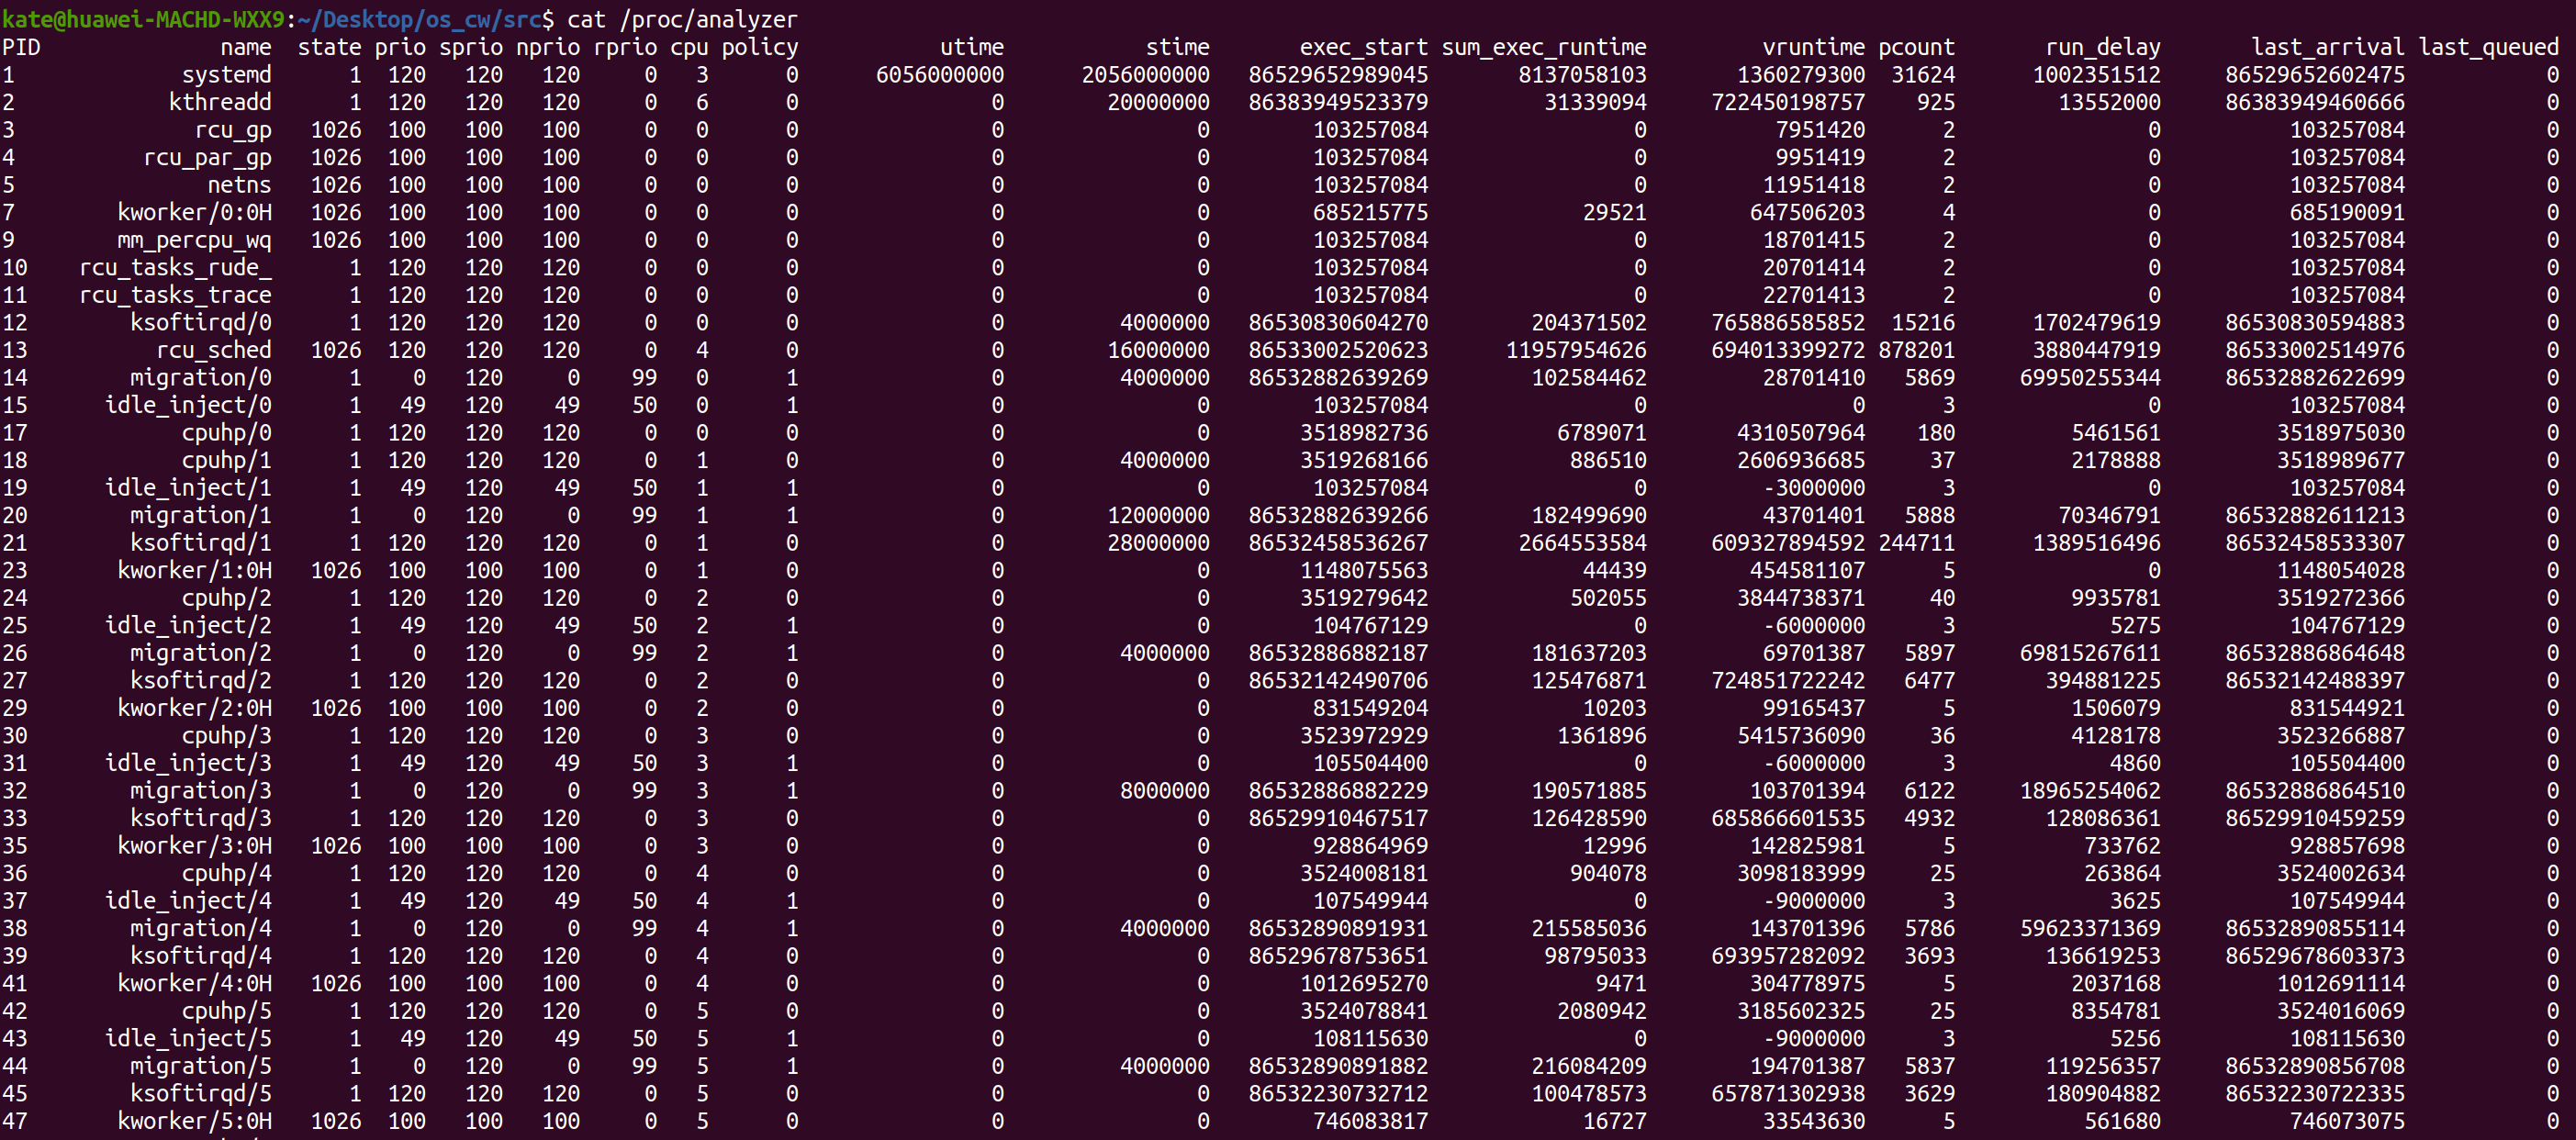
\includegraphics[width=\linewidth]{img/log.png}
% 	\caption{Результат работы модуля}
% 	\label{figlog}
% \end{figure}

% На рисунке \ref{figlogfilter} представлен пример вывода этого файла с фильтрацией по исполняющему ядру процессора.

% \begin{figure}[H]
% 	\centering
% 	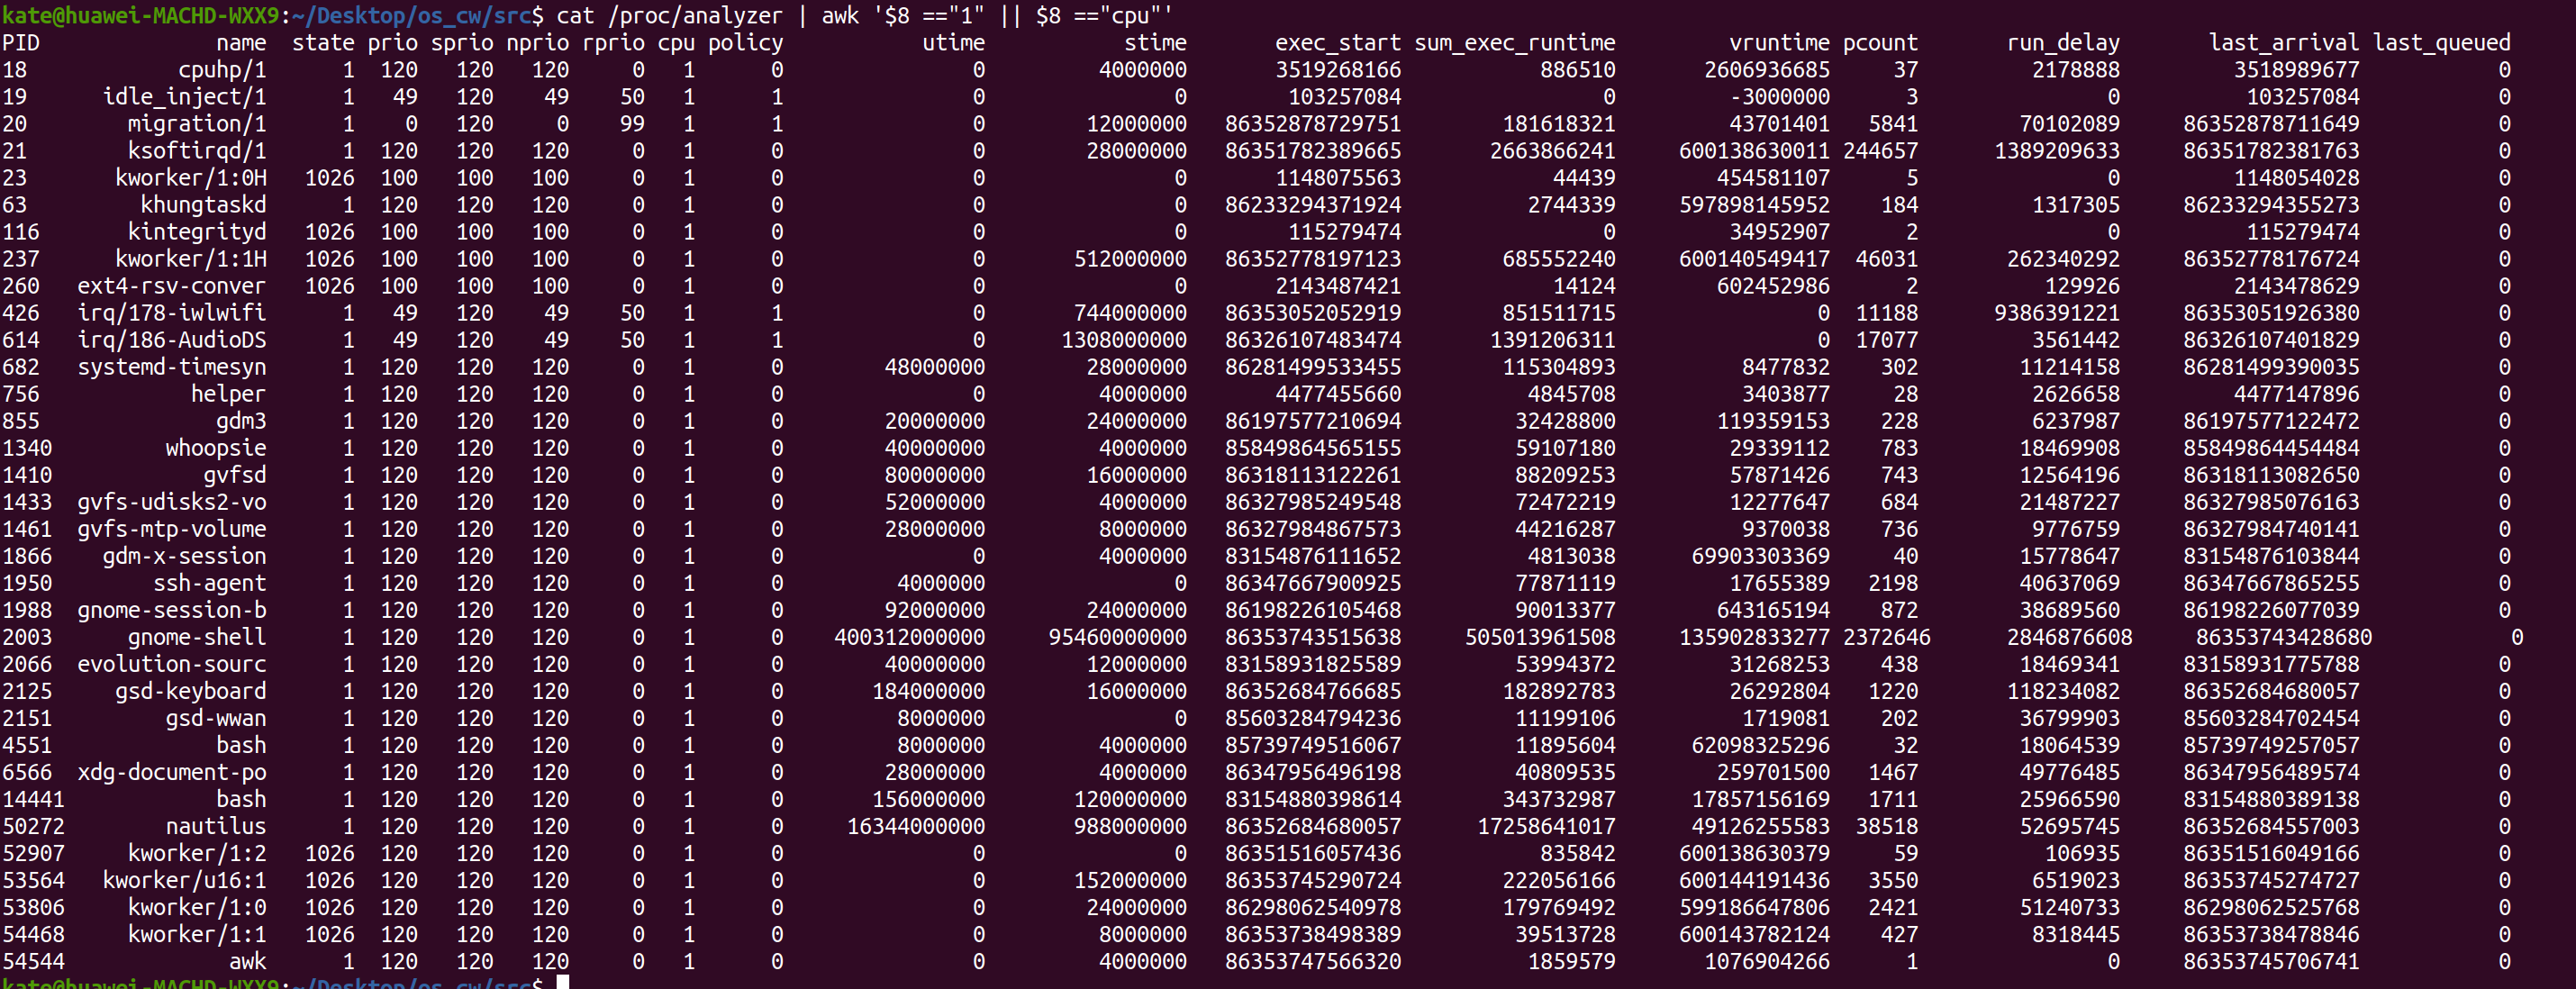
\includegraphics[width=\linewidth]{img/log_filter.png}
% 	\caption{Результат работы модуля с фильтрацией}
% 	\label{figlogfilter}
% \end{figure}

% На рисунке \ref{figwork} представлен процесс создания, загрузки модуля, работы с ним и выгрузки.
% \begin{figure}[H]
% 	\centering
% 	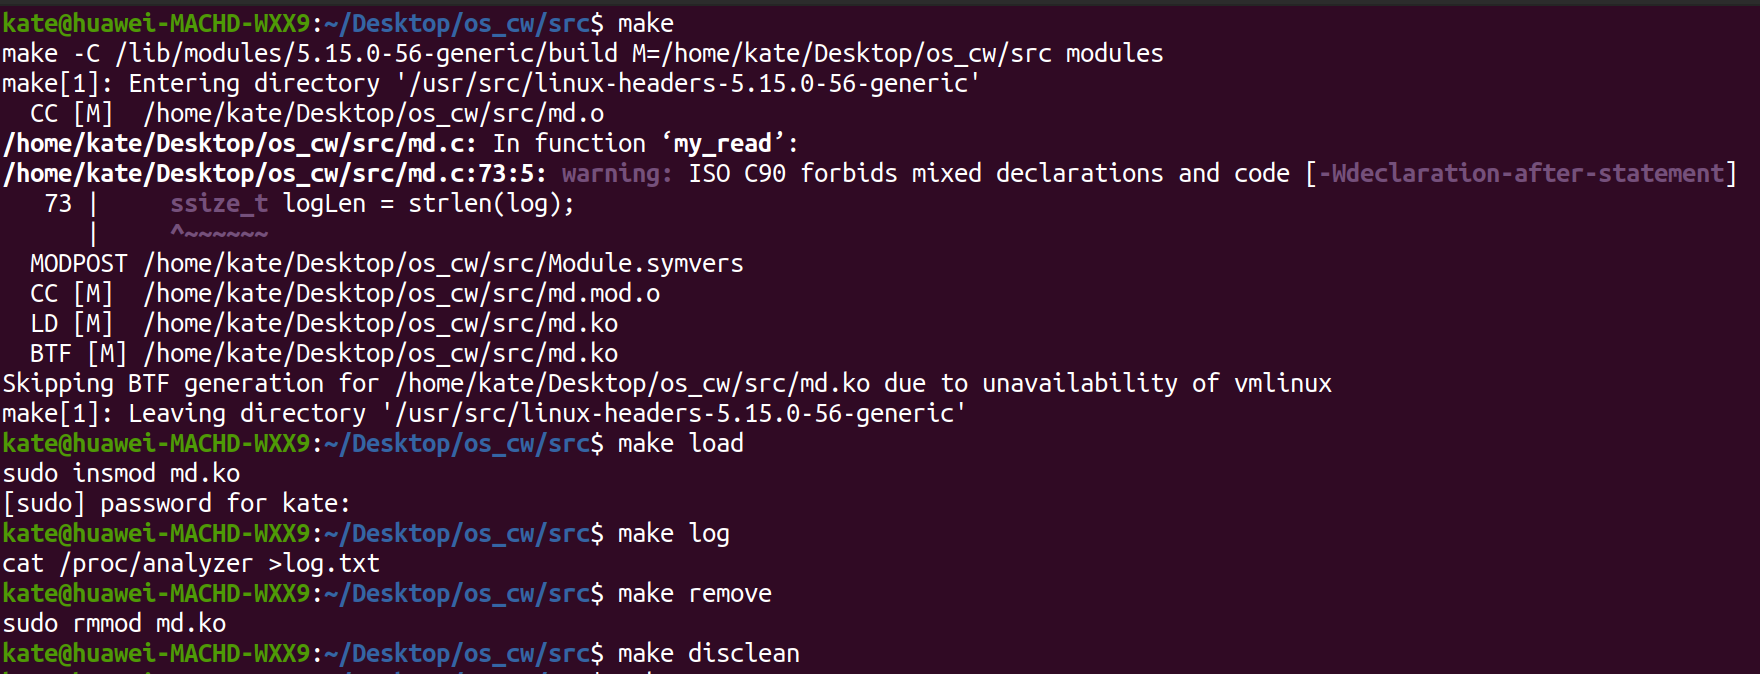
\includegraphics[width=\linewidth]{img/work.png}
% 	\caption{Процесс работы с модулем}
% 	\label{figwork}
% \end{figure}

\section*{Выводы}
В результате, был разработан модуль ядра Linux, реализующий мониторинг информации о процессах в соответствии с разработанными в конструкторском разделе алгоритмами, а также теоретическими сведениями о структурах ядра Linux, полученными в аналитическом разделе.